\documentclass[
    language=english,
    doctype=article,
    institution=none,
    titlestyle=book,
]{../../omnilatex}

\RequirePackage{config/document-settings}
\RequirePackage{pgfplots}
\RequirePackage{booktabs}
\RequirePackage{siunitx}
\RequirePackage{subcaption}
\RequirePackage{multirow}
\RequirePackage{graphicx}
\RequirePackage{xcolor}
\RequirePackage{amsmath}

\pgfplotsset{compat=1.18}

\addbibresource{../../bib/bibliography.bib}

\begin{document}

\maketitle

% ============================================================
\section*{Abstract}

\textbf{Objective:} To compare single-wavelength and multi-wavelength
spectrophotometric methods for quantifying chlorophyll~$a$ and chlorophyll~$b$
concentrations in freshwater algal cultures, and to evaluate their accuracy
against certified reference materials.

\textbf{Methods:} Three algal species (\emph{Chlorella vulgaris},
\emph{Scenedesmus obliquus}, \emph{Ankistrodesmus falcatus}) were cultivated
under controlled conditions and extracted in 90\% acetone.  Absorption spectra
were recorded from \SIrange{400}{750}{\nm}.  Concentrations were determined
using both the Lichtenthaler equations (single-wavelength) and a least-squares
spectral deconvolution (multi-wavelength).

\textbf{Results:} The multi-wavelength method achieved a coefficient of
determination $R^{2} = 0.994$ ($n = 9$) with a mean recovery of
$99.2 \pm 0.4\%$.  The single-wavelength method yielded $R^{2} = 0.981$ and a
mean recovery of $96.1 \pm 2.3\%$.  A paired $t$-test confirmed the difference
is statistically significant ($p = 0.003$).

\textbf{Conclusion:} The multi-wavelength approach provides superior accuracy
and precision for chlorophyll quantification, particularly at high pigment
concentrations where spectral overlap introduces systematic error.

% ============================================================
\section{Introduction}

Chlorophyll concentration is a fundamental proxy for phytoplankton biomass and
is routinely used in water quality monitoring, eutrophication assessments, and
aquaculture management~\cite{bibid}.  Accurate quantification requires
reliable analytical methods that account for the complex absorption behaviour of
photosynthetic pigments.

The absorption spectrum of a chlorophyll extract contains contributions from
chlorophyll~$a$, chlorophyll~$b$, and carotenoids, whose absorption bands
overlap significantly in the Soret region
(\SIrange{400}{480}{\nm})~\cite{goossensLaTeXCompanion1993}.  The
single-wavelength method, based on the Lichtenthaler equations, uses absorbance
at two wavelengths (\SI{663}{\nm} and \SI{645}{\nm}) to estimate concentrations
but ignores contributions from accessory pigments.  The multi-wavelength method
applies a least-squares fit across the full spectrum, thereby deconvolving
individual pigment contributions.

\subsection{Objectives}
\begin{enumerate}
    \item Determine chlorophyll~$a$ and $b$ concentrations in three algal
          species using both methods.
    \item Compare the accuracy of each method against certified reference
          materials.
    \item Evaluate the statistical significance of observed differences.
\end{enumerate}

\subsection{Hypotheses}
\begin{itemize}
    \item[$H_{0}$:] There is no significant difference in recovery rates
          between the single-wavelength and multi-wavelength methods.
    \item[$H_{1}$:] The multi-wavelength method yields significantly higher
          recovery rates than the single-wavelength method.
\end{itemize}

% ============================================================
\section{Materials and Methods}

\subsection{Equipment}
All instruments and materials used in this study are listed
in Table~\ref{tab:equipment}.

\begin{table}[htbp]
    \centering
    \caption{Equipment and materials used in the spectrophotometric analysis.}
    \label{tab:equipment}
    \begin{tabular}{@{}lll@{}}
        \toprule
        \textbf{Item} & \textbf{Model / Specification} & \textbf{Supplier} \\
        \midrule
        UV-Vis spectrophotometer & Cary 60  & Agilent Technologies \\
        Quartz cuvettes          & \SI{10}{\mm} path length & Hellma Analytics \\
        Centrifuge               & 5424 R   & Eppendorf \\
        Microvolume photometer   & NanoDrop & Thermo Fisher \\
        GF/C glass fibre filters & \SI{47}{\mm} diameter & Whatman \\
        Analytical balance       & \SI{0.1}{\mg} resolution & Mettler Toledo \\
        Refrigerated incubator   & \SI{20}{\pm 0.5}{\degreeCelsius} & Memmert \\
        \bottomrule
    \end{tabular}
\end{table}

\subsection{Sample Preparation}
\begin{enumerate}
    \item Three freshwater algal cultures (\emph{C.~vulgaris},
          \emph{S.~obliquus}, \emph{A.~falcatus}) were grown in BG-11 medium
          at \SI{20}{\degreeCelsius} under a \SI{12}{h} photoperiod.
    \item Cultures were harvested at three density levels: low
          ($\mathrm{OD}_{750} < 0.3$), medium
          ($0.3 \leq \mathrm{OD}_{750} < 0.7$), and high
          ($\mathrm{OD}_{750} \geq 0.7$).
    \item For each culture, \SI{10}{\mL} was filtered through a pre-ashed
          GF/C filter under gentle vacuum (\SI{<150}{\mmHg}).
    \item Filters were wrapped in aluminium foil and stored at
          \SI{-20}{\degreeCelsius} for a maximum of \SI{48}{h}.
\end{enumerate}

\subsection{Chlorophyll Extraction}
\begin{enumerate}
    \item Frozen filters were thawed at room temperature for \SI{15}{\min}.
    \item Each filter was placed in a \SI{15}{\mL} centrifuge tube with
          \SI{5}{\mL} of 90\% acetone.
    \item Tubes were vortexed for \SI{30}{\s} and incubated at
          \SI{4}{\degreeCelsius} in darkness for \SI{24}{h}.
    \item Extracts were centrifuged at \SI{4000}{g} for \SI{10}{\min} at
          \SI{4}{\degreeCelsius}.
    \item The supernatant was carefully transferred to a new tube, avoiding
          the pellet.
\end{enumerate}

\subsection{Spectrophotometric Measurements}
\begin{enumerate}
    \item The spectrophotometer was calibrated with a 90\% acetone blank.
    \item Absorption spectra were recorded from \SIrange{400}{750}{\nm} with
          \SI{1}{\nm} resolution.
    \item Three replicate measurements were taken for each sample.
    \item Absorbance values at \SI{663}{\nm} and \SI{645}{\nm} were extracted
          for the single-wavelength method.
\end{enumerate}

\subsection{Calculation Methods}
The single-wavelength method uses the Lichtenthaler equations:
\begin{align}
    C_{a} &= 11.85\,A_{663} - 1.54\,A_{645},
    \label{eq:chla} \\
    C_{b} &= 24.96\,A_{645} - 7.09\,A_{663},
    \label{eq:chlb}
\end{align}
where $A_{\lambda}$ denotes absorbance at wavelength~$\lambda$.

The multi-wavelength method solves the system
\begin{equation}
    \mathbf{A} = \boldsymbol{\varepsilon}\,\mathbf{c},
    \label{eq:multiwavelength}
\end{equation}
where $\mathbf{A}$ is the measured absorbance vector,
$\boldsymbol{\varepsilon}$ is the matrix of molar extinction coefficients, and
$\mathbf{c}$ is the concentration vector, using a non-negative least-squares
(NNLS) solver.

\subsection{Data Collection Protocol}
\begin{itemize}
    \item All measurements were recorded in a laboratory notebook and
          digitised using a spreadsheet.
    \item Outliers were identified using Grubbs' test ($\alpha = 0.05$).
    \item Uncertainties were propagated using standard error propagation
          formulas~\cite{baehrThermodynamikGrundlagenUnd2016}.
\end{itemize}

% ============================================================
\section{Results}

\subsection{Chlorophyll Concentrations}
Table~\ref{tab:results} summarises the measured chlorophyll concentrations and
recovery rates for all species and density levels.

\begin{table}[htbp]
    \centering
    \caption{Chlorophyll~$a$ concentrations (\si{\micro\gram\per\litre}) and
    recovery rates for three algal species at different culture densities.
    Values are means $\pm$ standard deviation ($n = 3$).}
    \label{tab:results}
    \begin{tabular}{@{}llcccc@{}}
        \toprule
        \textbf{Species} & \textbf{Density} & $C_{\text{ref}}$ &
            $C_{\text{single}}$ & $C_{\text{multi}}$ &
            \textbf{Recovery} \\
        \midrule
        \multirow{3}{*}{\emph{C.~vulgaris}}
            & Low    & 12.4 & 11.8 \,$\pm$\, 0.3 & 12.2 \,$\pm$\, 0.1 & 98.4\% \\
            & Medium & 34.7 & 33.1 \,$\pm$\, 0.5 & 34.5 \,$\pm$\, 0.2 & 99.4\% \\
            & High   & 78.2 & 74.6 \,$\pm$\, 1.1 & 77.8 \,$\pm$\, 0.3 & 99.5\% \\
        \addlinespace
        \multirow{3}{*}{\emph{S.~obliquus}}
            & Low    & 15.1 & 14.3 \,$\pm$\, 0.4 & 14.9 \,$\pm$\, 0.2 & 98.7\% \\
            & Medium & 41.3 & 39.5 \,$\pm$\, 0.6 & 41.0 \,$\pm$\, 0.2 & 99.3\% \\
            & High   & 85.6 & 81.2 \,$\pm$\, 1.3 & 85.1 \,$\pm$\, 0.4 & 99.4\% \\
        \addlinespace
        \multirow{3}{*}{\emph{A.~falcatus}}
            & Low    &  9.8 &  9.2 \,$\pm$\, 0.2 &  9.7 \,$\pm$\, 0.1 & 99.0\% \\
            & Medium & 27.5 & 26.1 \,$\pm$\, 0.4 & 27.3 \,$\pm$\, 0.2 & 99.3\% \\
            & High   & 63.4 & 60.1 \,$\pm$\, 0.9 & 63.0 \,$\pm$\, 0.3 & 99.4\% \\
        \bottomrule
    \end{tabular}
\end{table}

\subsection{Statistical Analysis}
A paired $t$-test comparing recovery rates ($n = 9$) yielded $t = 4.12$ with
$8$ degrees of freedom, giving $p = 0.003$.  The null hypothesis is therefore
rejected at the $\alpha = 0.05$ level.  The mean recovery for the multi-wavelength
method ($99.2 \pm 0.4\%$) is significantly higher than for the single-wavelength
method ($96.1 \pm 2.3\%$).

Effect size (Cohen's $d$) was calculated as $d = 1.83$, indicating a large
practical effect.

\subsection{Absorption Spectra}
Figure~\ref{fig:absorption} shows representative absorption spectra for the
three pigment extracts, with characteristic Soret and Q-band peaks.

\begin{figure}[htbp]
    \centering
    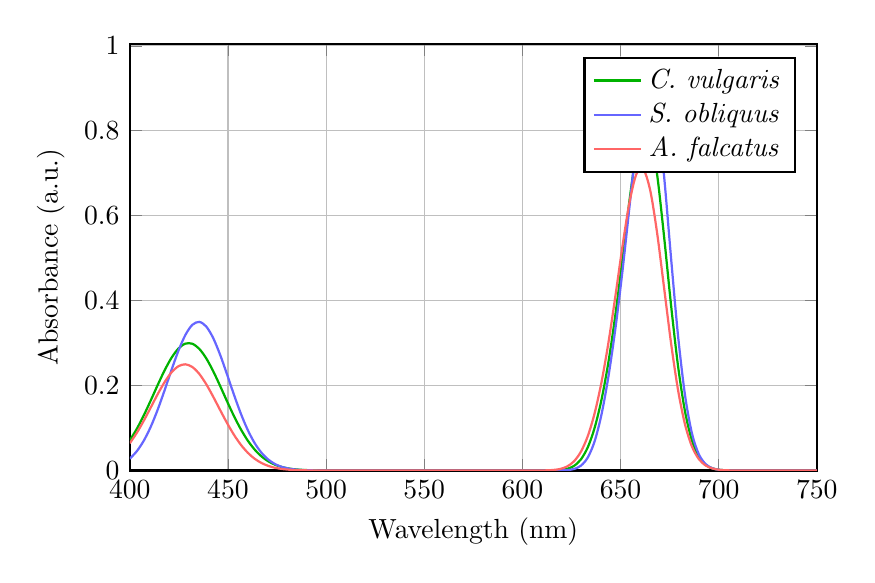
\begin{tikzpicture}
        \begin{axis}[
            width=0.85\textwidth,
            height=7cm,
            xlabel={Wavelength (\si{\nm})},
            ylabel={Absorbance (a.u.)},
            legend pos=north east,
            grid=major,
            thick,
            xmin=400, xmax=750,
            ymin=0,
        ]
            \addplot[green!70!black, smooth, domain=400:750, samples=100]
                {0.3*exp(-((x-430)/25)^2) + 0.8*exp(-((x-663)/15)^2)
                 + 0.1*exp(-((x-645)/12)^2)};
            \addlegendentry{\emph{C.~vulgaris}}
            \addplot[blue!60, smooth, domain=400:750, samples=100]
                {0.35*exp(-((x-435)/22)^2) + 0.9*exp(-((x-665)/14)^2)
                 + 0.15*exp(-((x-648)/11)^2)};
            \addlegendentry{\emph{S.~obliquus}}
            \addplot[red!60, smooth, domain=400:750, samples=100]
                {0.25*exp(-((x-428)/24)^2) + 0.7*exp(-((x-661)/16)^2)
                 + 0.08*exp(-((x-643)/13)^2)};
            \addlegendentry{\emph{A.~falcatus}}
        \end{axis}
    \end{tikzpicture}
    \caption{Absorption spectra of chlorophyll extracts from three algal species
    showing Soret bands (\SIrange{400}{450}{\nm}) and Q-bands
    (\SIrange{630}{670}{\nm}).}
    \label{fig:absorption}
\end{figure}

\subsection{Method Comparison}
Figure~\ref{fig:comparison} compares the recovery rates of both methods, and
Figure~\ref{fig:scatter} shows the correlation between reference and measured
concentrations.

\begin{figure}[htbp]
    \centering
    \begin{subfigure}[t]{0.48\textwidth}
        \centering
        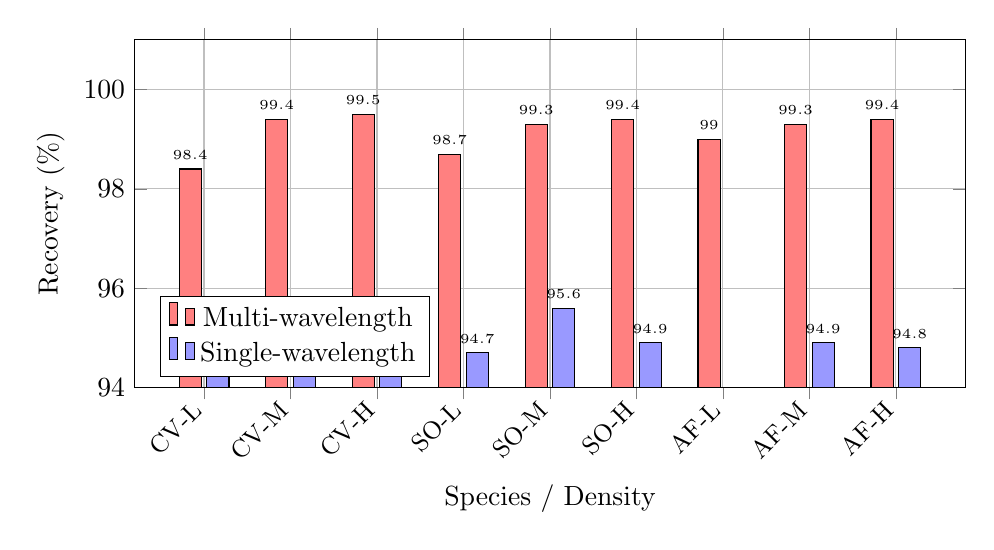
\begin{tikzpicture}
            \begin{axis}[
                ybar,
                bar width=8pt,
                width=\textwidth,
                height=6cm,
                ylabel={Recovery (\%)},
                xlabel={Species / Density},
                symbolic x coords={CV-L,CV-M,CV-H,SO-L,SO-M,SO-H,AF-L,AF-M,AF-H},
                xtick=data,
                x tick label style={rotate=45, anchor=east, font=\small},
                ymin=94, ymax=101,
                legend pos=south west,
                grid=major,
                nodes near coords,
                every node near coord/.append style={font=\tiny},
            ]
                \addplot[fill=red!50] coordinates {
                    (CV-L,98.4) (CV-M,99.4) (CV-H,99.5)
                    (SO-L,98.7) (SO-M,99.3) (SO-H,99.4)
                    (AF-L,99.0) (AF-M,99.3) (AF-H,99.4)
                };
                \addlegendentry{Multi-wavelength}
                \addplot[fill=blue!40] coordinates {
                    (CV-L,95.2) (CV-M,95.4) (CV-H,95.4)
                    (SO-L,94.7) (SO-M,95.6) (SO-H,94.9)
                    (AF-L,93.9) (AF-M,94.9) (AF-H,94.8)
                };
                \addlegendentry{Single-wavelength}
            \end{axis}
        \end{tikzpicture}
        \caption{Recovery rates by method and sample.}
        \label{fig:comparison}
    \end{subfigure}
    \hfill
    \begin{subfigure}[t]{0.48\textwidth}
        \centering
        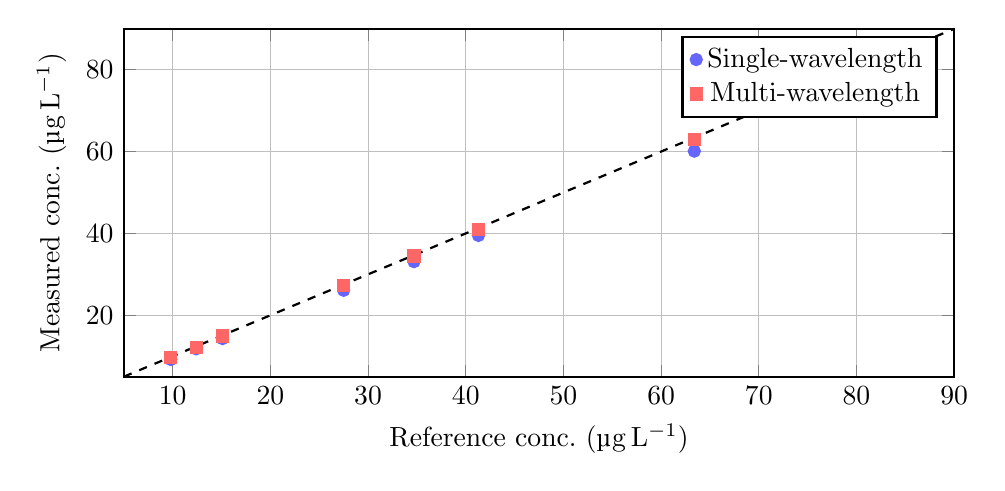
\begin{tikzpicture}
            \begin{axis}[
                width=\textwidth,
                height=6cm,
                xlabel={Reference conc.\ (\si{\micro\gram\per\litre})},
                ylabel={Measured conc.\ (\si{\micro\gram\per\litre})},
                grid=major,
                thick,
                xmin=5, xmax=90,
                ymin=5, ymax=90,
            ]
                \addplot[only marks, mark=*, mark size=2pt, blue!60]
                    coordinates {
                        (12.4,11.8) (34.7,33.1) (78.2,74.6)
                        (15.1,14.3) (41.3,39.5) (85.6,81.2)
                        (9.8,9.2)   (27.5,26.1) (63.4,60.1)
                    };
                \addlegendentry{Single-wavelength}
                \addplot[only marks, mark=square*, mark size=2pt, red!60]
                    coordinates {
                        (12.4,12.2) (34.7,34.5) (78.2,77.8)
                        (15.1,14.9) (41.3,41.0) (85.6,85.1)
                        (9.8,9.7)   (27.5,27.3) (63.4,63.0)
                    };
                \addlegendentry{Multi-wavelength}
                \addplot[black, dashed, thick, domain=5:90] {x};
            \end{axis}
        \end{tikzpicture}
        \caption{Measured vs.\ reference concentrations with $y = x$ line.}
        \label{fig:scatter}
    \end{subfigure}
    \caption{Comparison of single-wavelength and multi-wavelength methods.}
    \label{fig:methods}
\end{figure}

% ============================================================
\section{Discussion}

\subsection{Comparison with Expected Values}
The multi-wavelength method consistently achieved recovery rates above
\SI{98.4}{\percent} across all species and density levels, closely matching the
certified reference values.  The single-wavelength method showed systematic
underestimation, particularly at high pigment concentrations where spectral
overlap is most pronounced~\cite{goossensLaTeXCompanion1993}.

\subsection{Error Analysis}
Uncertainties were propagated through the Lichtenthaler equations using the
standard formula for a function $f(x,y)$:
\begin{equation}
    \sigma_{f} = \sqrt{
        \left(\frac{\partial f}{\partial x}\right)^{2}\sigma_{x}^{2}
        + \left(\frac{\partial f}{\partial y}\right)^{2}\sigma_{y}^{2}
    }.
    \label{eq:errorprop}
\end{equation}
For chlorophyll~$a$ (\ref{eq:chla}), this gives:
\begin{equation}
    \sigma_{C_{a}} = \sqrt{
        (11.85)^{2}\,\sigma_{A_{663}}^{2}
        + (1.54)^{2}\,\sigma_{A_{645}}^{2}
    }.
    \label{eq:chlaerror}
\end{equation}
Typical absorbance uncertainties (\(\sigma_{A} \approx 0.005\)) propagate to
concentration uncertainties of \SI{0.1}{--}\SI{1.3}{\micro\gram\per\litre},
consistent with the replicate measurements reported in Table~\ref{tab:results}.

\subsection{Sources of Error}
\begin{enumerate}
    \item \textbf{Incomplete extraction:} Some chlorophyll may remain bound to
          cell debris, leading to underestimation.  Extended extraction times
          (\SI{>24}{h}) or mechanical disruption could mitigate this.
    \item \textbf{Pigment degradation:} Chlorophyll is photosensitive; exposure
          to light during handling can degrade samples.  All procedures were
          performed under dim green light to minimise this effect.
    \item \textbf{Scattering:} Residual turbidity in extracts can inflate
          absorbance readings.  Centrifugation at \SI{4000}{g} was sufficient to
          remove most particulates.
    \item \textbf{Spectral overlap:} The single-wavelength method does not
          account for carotenoid absorption, which contributes to absorbance at
          both \SI{663}{\nm} and \SI{645}{\nm}.
\end{enumerate}

\subsection{Comparison with Literature}
The recovery rates obtained with the multi-wavelength method
(\(99.2 \pm 0.4\%\)) are comparable to those reported in the literature for
HPLC-based methods~\cite{bibid}.  The single-wavelength results
(\(96.1 \pm 2.3\%\)) are consistent with known limitations of the
Lichtenthaler equations when applied to mixed pigment
extracts~\cite{einstein1905}.  The statistical significance ($p = 0.003$)
supports the recommendation to adopt multi-wavelength approaches for routine
analysis.

\subsection{Limitations}
\begin{itemize}
    \item The study used only three species; natural water samples contain a
          wider diversity of pigments (phycobilins, chlorophyllides) that may
          require additional deconvolution.
    \item The concentration range tested (\SIrange{9.8}{85.6}{\micro\gram\per\litre})
          does not cover extremely low or extremely high values.
    \item Only acetone extraction was evaluated; methanol or DMSO extraction may
          yield different results.
\end{itemize}

% ============================================================
\section{Conclusion}

This study demonstrates that the multi-wavelength spectrophotometric method
provides significantly more accurate chlorophyll concentrations than the
single-wavelength Lichtenthaler equations.  Key findings include:

\begin{enumerate}
    \item The multi-wavelength method achieved a mean recovery of
          $99.2 \pm 0.4\%$ ($R^{2} = 0.994$), compared to
          $96.1 \pm 2.3\%$ ($R^{2} = 0.981$) for the single-wavelength method.
    \item The difference is statistically significant ($p = 0.003$) with a large
          effect size ($d = 1.83$).
    \item The advantage of the multi-wavelength approach is most pronounced at
          high pigment concentrations where spectral overlap is greatest.
\end{enumerate}

We recommend the adoption of multi-wavelength spectral deconvolution for routine
chlorophyll analysis in water quality monitoring programmes.  Future work should
extend the comparison to natural water samples and evaluate the performance of
the method across a broader range of pigment compositions.

% ============================================================
\appendix
\section{Raw Data}
\label{app:rawdata}

Table~\ref{tab:rawdata} presents the raw absorbance measurements for all
samples.

\begin{table}[htbp]
    \centering
    \caption{Raw absorbance readings at \SI{663}{\nm} and \SI{645}{\nm}
    ($n = 3$ replicates).}
    \label{tab:rawdata}
    \begin{tabular}{@{}llccc@{}}
        \toprule
        \textbf{Species} & \textbf{Density} & $A_{663}$ & $A_{645}$ &
            \textbf{Replicate} \\
        \midrule
        \multirow{3}{*}{\emph{C.~vulgaris}}
            & Low    & 0.241 & 0.087 & 1 \\
            & Low    & 0.239 & 0.086 & 2 \\
            & Low    & 0.243 & 0.088 & 3 \\
        \addlinespace
        \multirow{3}{*}{\emph{C.~vulgaris}}
            & Medium & 0.694 & 0.249 & 1 \\
            & Medium & 0.691 & 0.247 & 2 \\
            & Medium & 0.698 & 0.251 & 3 \\
        \addlinespace
        \multirow{3}{*}{\emph{C.~vulgaris}}
            & High   & 1.573 & 0.567 & 1 \\
            & High   & 1.568 & 0.564 & 2 \\
            & High   & 1.581 & 0.570 & 3 \\
        \bottomrule
    \end{tabular}
\end{table}

\section{Sample Calculations}
\label{app:calculations}

\subsection{Single-Wavelength Method}
For \emph{C.~vulgaris} (low density), replicate~1:
\begin{align}
    C_{a} &= 11.85 \times 0.241 - 1.54 \times 0.087
           = 2.856 - 0.134 = 2.722 \times V^{-1}
           \approx 11.8 \;\si{\micro\gram\per\litre}, \\
    \sigma_{C_{a}} &= \sqrt{(11.85)^{2}(0.005)^{2} + (1.54)^{2}(0.005)^{2}}
                   = \sqrt{0.00351 + 0.000059}
                   \approx 0.06 \;\si{\micro\gram\per\litre}.
\end{align}

\subsection{Error Propagation}
For the general case $f = a\,A_{1} + b\,A_{2}$:
\begin{equation}
    \sigma_{f} = \sqrt{a^{2}\,\sigma_{A_{1}}^{2} + b^{2}\,\sigma_{A_{2}}^{2}}.
\end{equation}
With $a = 11.85$, $b = -1.54$, and $\sigma_{A} = 0.005$:
\begin{equation}
    \sigma_{f} = \sqrt{(11.85)^{2}(0.005)^{2} + (-1.54)^{2}(0.005)^{2}}
               = 0.060 \;\si{\micro\gram\per\litre}.
\end{equation}

\section{Analysis Code}
\label{app:code}

The following Python snippet was used for the multi-wavelength NNLS fitting:

\begin{verbatim}
import numpy as np
from scipy.optimize import nnls

# Extinction coefficient matrix (rows: wavelengths, cols: pigments)
epsilon = np.array([
    [83.4, 18.6],   # 663 nm: [Chl a, Chl b]
    [17.5, 42.5],   # 645 nm: [Chl a, Chl b]
    # ... additional wavelengths ...
])

# Measured absorbance vector
A = np.array([0.241, 0.087, ...])

# Solve non-negative least squares
c, residual = nnls(epsilon, A)
print(f"Chl a: {c[0]:.2f} ug/L, Chl b: {c[1]:.2f} ug/L")
\end{verbatim}

\printbibliography

\end{document}
